\documentclass[../main.tex]{subfiles}
\begin{document}
\setchapterstyle{kao}
\setchapterpreamble[u]{\margintoc}
\chapter[Lie groups III - Topological properties]{Lie groups III - Topological properties\footnotemark[0]}
\labch{Lie-groups-III}
%INIZIO LEZIONE 13 - 21/04/2022
First of all, we should say under which conditions we identify two Lie groups (this is very typical of mathematics).
\section{Homo- and iso-morphisms of Lie groups}
\begin{definition}[Homomorphism of Lie groups]\index{Homomorphism of Lie groups}
Let $G$ and $H$ be Lie groups. A \textbf{homomorphism of Lie groups} is a map $\varphi: \ G\to H$ such that:
\begin{enumerate}
    \item $\varphi$ is a \textbf{homomorphism of groups}, i.e.\marginnote{Pedantic notation
    \[
    \varphi(g_1\ast_G g_2)&=\varphi(g_1)\ast_H \varphi(g_2)
    \]}
    \[
    \varphi(g_1g_2)=\varphi(g_1)\varphi(g_2) \quad \forall \ g_1,g_2 \in G
    \]
    \item $\varphi$ is $C^\infty$\textbf{-smooth}
\end{enumerate}
\end{definition}
\begin{example}
Take the general linear group in the complex numbers, you have an homomorphism to invertible complex numbers (minus 0), which is very well-known:
\[
\begin{split}
    \det: \ \textrm{GL}(n,\mathbb{C}) &\to \mathbb{C}^\times = \mathbb{C}\setminus \Bqty{0}\\
    A & \mapsto \det (A)
\end{split}
\]
Let us check that it is an homomorphism:
\begin{enumerate}
    \item $\det(AB)\overset{\mathclap{\tikz \node {$\downarrow$} node [above=1.25ex] {\footnotesize Binet};}}{=}\det(A)\cdot\det(B) \quad \quad$ ok \checkmark
    \item $\det(A)$ is a polynomial in the entries of $A$, i.e. the coordinates $x^\mu (A)=A^i_{\; j}$ with $\mu = (i,j)$ and a polynomial are $C^\infty$\textbf{-smooth.}
\end{enumerate}
\end{example}
\begin{example}
Take\marginnote{There was an erratum: the example here must be downgraded to dimension one, because otherwise is not true that the exponential of a sum is the product of the exponential, unless the matrix commute. So either we restrict to space of commuting endomorphism or we consider it in dimension one.}
\[
\begin{split}
\exp: \left(\mathbb{C}, + \right) &\to \left(\mathbb{C}^\times, \circ \right)\\
A & \mapsto e^A
\end{split}
\]
This is a \textbf{homomorphism of Lie groups.}
\end{example}
\begin{definition}[Isomorphism of Lie groups]\index{Isomorphism of Lie groups}
Let $G$ and $\Tilde{G}$ be Lie groups. An \textbf{isomorphism of Lie groups} is a map $\varphi: \ G\to \tilde{G}$ which is \textbf{bijective} and:\marginnote{Notice that the second property is not automatic!! The inverse of a smooth map has no reason to be a smooth map.}
\begin{enumerate}
    \item $\varphi$ is a homomorphism of Lie groups
    \item $\varphi^{-1}$ is a homomorphism of Lie groups
\end{enumerate}
\end{definition}
\begin{kaobox}[frametitle=Notation]
If there is an isomorphism of Lie groups we write
\[
G \xrightarrow[\textrm{Lie}]{\cong} \Tilde{G} \quad \textrm{or shortly} \quad G\underset{\textrm{Lie}}{\cong} \Tilde{G}
\]
Most of the books do not put the word \textit{Lie} below.
\end{kaobox}
Let us emphasize that
\[
\text{\parbox{4 cm}{\centering isomorphism of \\[-4pt]  Lie groups}}\textbf{stronger} \text{\parbox{4 cm}{\centering isomorphism \\[-4pt]  of groups}}
\]
the isomorphism of groups guarantees that the two algebraic structures are identified, but it does not say anything about the differentiable structures. This is why the professor prefers to put the word \textit{Lie} below. Now we are ready to define what are matrix Lie groups.
\section{Matrix Lie groups}
In simple words they are Lie groups which consist of matrices, but with a \textit{\href{https://it.wikipedia.org/wiki/Caveat}{caveat}}\sidenote{\textit{Caveat} espressione latina (terza persona del congiuntivo presente del verbo \textit{cavere}: "stia attento"); al plurale \textit{caveant}.}: it might be that they are not given as group of matrices, but they are isomorphic to a group of matrices.
\begin{definition}[Matrix Lie group]\index{Matrix Lie group}A Lie group $G$ is a \textbf{matrix Lie group} if it is isomorphic to a Lie subgroup of $\textrm{GL}(N,\mathbb{C})$ \textbf{for some $N\in\mathbb{N}^\ast$.}
\end{definition}
Basically all the examples we have seen so far are matrix Lie groups: the orthogonal group and the unitary group were already given as group of matrices\sidenote{Maybe we defined them as group of endomorphism, but as soon as we fix a linear basis in our linear space, the endomorphism corresponds to matrices. So they were already groups of matrices.}, while a few of them, the Euclidean group and the generalized Poincaré group in the \refsec{Euclidean-and-Poincaré-group}, were not given as group of matrices.
\begin{example}
All the previous examples (\refch{Lie-groups-I} and \refch{Lie-groups-II}). 

Notice that the Euclidean group is not itself a group of matrices, but it is isomorphic to the subgroup of the general linear group
\[
E(n) \xrightarrow[\textrm{Lie}]{\cong}H \subseteq \textrm{GL}({\color{red}n+1}, \mathbb{R})
\]
where (in dimension three) 
\[
H=\Bqty{
\left(
\begin{array}{ccc:c}
& & & a_1\\
& \bigR & & a_2\\
& & & a_3\\
\hdashline
0&0&0 &1\\
\end{array}
\right) \ : R\in \textrm{SO}(3), \ni \hat{\mathbb{R}}^3
}
\]
even the Euclidean group (and the Poincaré group), which are not defined as groups of matrices, are actually matrix Lie groups. This is a very general class.
\end{example}
\underline{Question}: is every Lie group a matrix Lie group?

\underline{Answer}: No. \raisebox{-\mydepth}{{
\includegraphics[height=1.1\baselineskip]{images/sadsmile.jpg}}}

Counter example: a very simple example is one in a sense inspired by the Heisenberg group\sidenote{\href{https://en.wikipedia.org/wiki/Heisenberg_group}{Heisenberg group}: in mathematics, the \textbf{Heisenberg group} $H$, named after Werner Heisenberg, is the group of $3\times 3$ upper triangular matrices of the form
\[\begin{pmatrix}
 1 & a & c\\
 0 & 1 & b\\
 0 & 0 & 1\\
\end{pmatrix}
\]
under the operation of matrix multiplication. Elements $a, b$ and $c$ can be taken from any commutative ring with identity, often taken to be the ring of real numbers (resulting in the "continuous Heisenberg group") or the ring of integers (resulting in the "discrete Heisenberg group").}. Consider:
\[
\begin{split}
G&=\mathbb{R}\times \mathbb{R}\times \textrm{U}(1)\\
G&\ni (x,y,u)
\end{split}
\]
where $\textrm{U}(1)$ are unimodular complex numbers. But the product is a bit twisted\sidenote{If this reminds you of punctuation relations in QM, it is because it is a good analogy. It is not the same thing, but you can describe it with that.}
\[
(x_1,y_1,u_1)\underset{\mathclap{\tikz \node {$\uparrow$} node [below=1ex] {\footnotesize In $G$ };}}{\cdot}(x_2,y_2,u_2) := (x_1+x_2, y_1+y_2, {\color{red}e^{ix}u_1u_2})
\]
\begin{starredExercise}
You can do this exercise after we do the representation theory [\refch{RT}].
\begin{enumerate}
    \item Prove that $G$ is a Lie group [easy].
    \item Prove that $G$ is \underline{\underline{\textbf{not}}} isomorphic to any subgroup of $\textrm{GL}(N,\mathbb{C})$ for any $N\in\mathbb{N}^\ast$. [Requires \textbf{representation theory}!\footnote{You will do it by contradiction, when we know that representation theory as/are matrix Lie groups ???}].
\end{enumerate}
\end{starredExercise}
\section{Topological properties of Lie groups}
We want to make an overview of some properties (compactness, connectedness and simple connectedness) and then we will study more in detail specific examples.
\subsection{Compactness}
\begin{definition}[Compactness (\textit{Compattezza)} for matrix Lie group]\index{Compactness for matrix Lie group}\footnote{We could give a general definition, but instead we will specialize to matrix Lie group}A matrix Lie group $G\leq \textrm{GL}(n,\mathbb{C}) \subseteq \mathbb{C}^{n^2}$ is \textbf{compact} if it is compact as a subset of $\mathbb{C}^{n^2}$.
\end{definition}
We will not see the general definition, but definition of compact that we saw in \textit{Analisi vettoriale} in the bachelor degree (\href{https://it.wikipedia.org/wiki/Spazio_compatto#Compattezza_di_spazi_euclidei}{compact} = close and bounded) is true only in finite dimensional space, and it is actually a theorem, indeed:
\begin{marginfigure}[-20mm]
	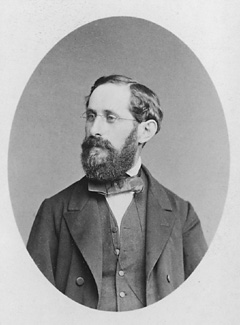
\includegraphics[width=1\linewidth]{images/Heinrich_Eduard_Heine_1.jpg}
	\caption[Heinrich Eduard Heine (1821-1881). Circa 1881]{From \href{https://commons.wikimedia.org/wiki/File:Heinrich_Eduard_Heine_1.jpg}{Wikimedia}: Heinrich Eduard Heine in circa 1881. Heinrich Eduard Heine (16 March 1821 – October 1881) was a German mathematician. Heine became known for results on special functions and in real analysis. In particular, he authored an important treatise on spherical harmonics and Legendre functions (\textit{Handbuch der Kugelfunctionen}). He also investigated basic hypergeometric series. He introduced the Mehler–Heine formula.}
	\labfig{Heine}
\end{marginfigure}
\begin{theorem}[\href{https://it.wikipedia.org/wiki/Teorema_di_Heine-Borel}{Heine-Borel}]\index{Heine-Borel}
\labthm{closedbounded}
A subset of $\mathbb{R}^N$ or $\mathbb{C}^N$ is \textbf{compact} (according to the general definition)
 if and only if it is \textbf{closed} and \textbf{bounded}.
\end{theorem}
\underline{Question:} Closed and bounded require, for example, a norm. To say that a set is bounded, we would say that the \href{https://it.wikipedia.org/wiki/Estremo_superiore_e_estremo_inferiore}{supremum} on the norm of all its elements is smaller than a constant. So we would need a norm, or at least the notion of a distance to say that is bounded. Hence the question is: in which sense \textbf{\textit{bounded}} is meant? With respect to which norm?

This question is not trivial if we are talking about endomorphisms, because suppose that $A\in \textrm{End}(\mathbb{R}^n)$, but the endomorphism on/of $\mathbb{R}^n$ are also real matrices $n\times n$ and, if we forget the multiplication structure, these are also elements of the linear space $\mathbb{R}^{n^2}$
\[
A\in \textrm{End}(\mathbb{R}^n)\simeq \textrm{Mat}(n,\mathbb{R})\simeq \mathbb{R}^{n^2}
\]
But we can consider different norms. 
\begin{enumerate}
    \item For example some authors (like Brian Hall, author of \sidecite{Hall2015}) consider the \href{https://it.wikipedia.org/wiki/Operatore_di_Hilbert-Schmidt}{Hilbert-Schmidt} norm:
    \begin{marginfigure}
	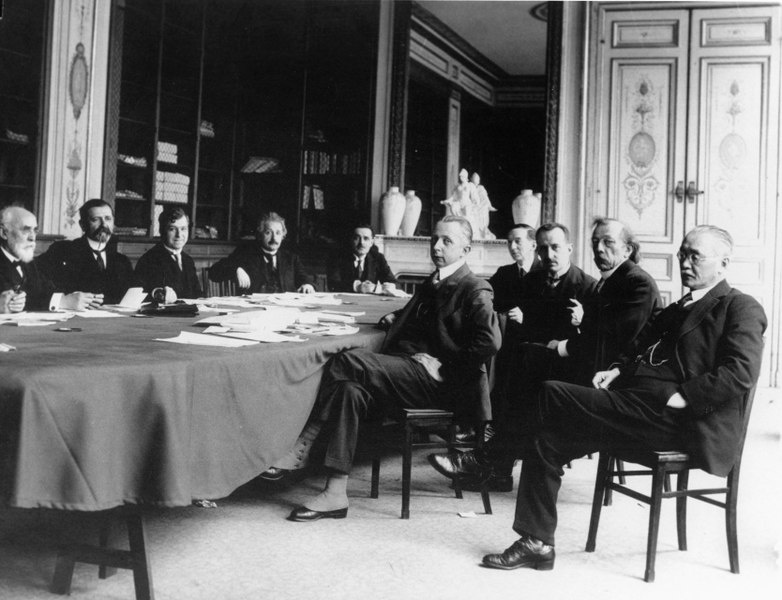
\includegraphics[width=1\linewidth]{images/lossy-page1-782px-League_of_Nations_Commission_067.tif.jpg}
	\caption[ International Committee on Intellectual Cooperation (League of Nations). Plenary session in the Palais Wilson, between 1924 and 1927.]{From \href{https://commons.wikimedia.org/wiki/File:League_of_Nations_Commission_067.tif?uselang=it}{Wikimedia}:  International Committee on Intellectual Cooperation (League of Nations). Plenary session in the Palais Wilson, between 1924 and 1927. Borel is the second person on the left. Félix Édouard Justin Émile Borel (7 January 1871 – 3 February 1956) was a French mathematician and politician. As a mathematician, he was known for his founding work in the areas of measure theory and probability.}
	\labfig{Borel}
\end{marginfigure}
    \[
    \norm{A}_{\textrm{HS}}=\sum_{i,j=1}^n\abs{A^i_{\;j}}^2 \quad \text{is a norm in $\text{End}(\mathbb{R}^n)$}
    \]
    One could prove that it is a norm and so it is compatible with the operations in the linear space.
    \item On the other hand we would also like another norm:
    \[
    \norm{A}=\sup_{\text{\parbox{0.8 cm}{\centering $x\neq 0$ \\[-4pt] $x\in\mathbb{R}^n$}}}\frac{\norm{Ax}}{\norm{x}} \quad \text{is a norm in $\text{End}(\mathbb{R}^n)$}
    \]
\end{enumerate}
We actually prefer the second choice because it has a natural generalization to infinite dimensional linear spaces. Apparently the question might be nasty, because every time we should specify bounded with respect to which norm, luckily there is a very nice lemma:
\begin{lemma}
Let $V$ a linear space over $\mathbb{K}\in\Bqty{\mathbb{R},\mathbb{C}}$ with $\dim V<+\infty$. Then \textbf{"all the norms are equivalent"}, namely: if $\norm{\dots}_1$ and $\norm{\dots}_2$ are two norms, $\exists \ c,C$ such that
\[
c\norm{v}_1\leq\norm{v}_2\leq C\norm{v}_1
\]
\end{lemma}
\underline{Answer:} It does not matter, all \textbf{norms are equivalent} (in the sense above) as far as $\dim \text{End}(\mathbb{R}^n)=n^2<+\infty$.\marginnote[-10mm]{If we had instead the group of unitary operators on an infinite dimensional Hilbert space, then the choice of norm would make a difference.}

\underline{\textbf{Examples}}

Among the families we have already considered, the examples of compact Lie groups are those associated to isometries of a real or complex inner product.

\underline{\textbf{Compact}}\marginnote[-20mm]{Essentially, the groups that are compact are those who are isometries of a real, or respectively complex, scalar product. Also the spin-n group is also related to the isometries of some sort of vector spaces, which are however over quaternions (\textit{\href{https://it.wikipedia.org/wiki/Quaternione}{quaternioni}}), not over fields of real or complex numbers. In mathematics, the \textbf{quaternion} number system extends the complex numbers. Quaternions were first described by Irish mathematician William Rowan Hamilton in 1843 as the quotient of two \textit{directed lines} in a three-dimensional space, or, equivalently, as the quotient of two vectors. Multiplication of quaternions is non commutative. Quaternions are generally represented in the form
:\[a + b\ \mathbf i + c\ \mathbf j +d\ \mathbf k\]
where $a, b, c$, and $d$ are real numbers; and \textbf{i}, \textbf{j}, and \textbf{k} are the \textit{basic quaternions}.}
\[
\begin{rcases}
\textrm{SO}(n),\; \textrm{O}(n)\\
\textrm{SU}(n),\; \textrm{U}(n)\\
\text{S}_\text{P}(n)
\end{rcases}
\textrm{ are compact}
\]
They are all \textbf{closed} subgroups of the general linear group (we already know that) $\textrm{GL}(n,\mathbb{K})$ (for the first four cases) or $\textrm{GL}(2n, \mathbb{K})$ (for the simplectic group). Moreover, they are \textbf{bounded}. 
We will not prove that for each family, but let us make an example considering the unitary group, take $U\in \textrm{U}(n)$. Consider the operator norm, we know that the norm is equal to the spectral radius
\[
\norm{U}=1
\]
How do we know that? We could use the following lemma.

\begin{kaobox}[frametitle=Remark]
If $A\in \textrm{End}(\mathbb{C})$ such that $AA^\ast=A^\ast A$ then\marginnote{e.v. = eigenvalue}
\begin{equation}\labeq{sp-radius}
\norm{A}= \sup_{\text{\parbox{0.8 cm}{\centering $\lambda$ e.v. \\[-4pt] of $A$}}}\abs{\lambda}=: \ \text{\parbox{0.8 cm}{\centering spectral \\[-4pt] radius}}
\end{equation}
\end{kaobox}
\begin{marginfigure}
	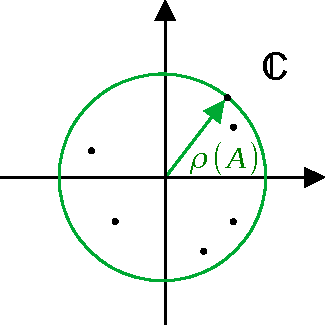
\includegraphics[width=1\linewidth]{images/autovalori_oper.pdf}
	\caption{Representation of the spectral radius.}
	\labfig{auto-op}
\end{marginfigure}
We basically look at the eigenvalues in the complex plane (the operator is not self-adjoint) and then we take the smallest circle which contains all of them, this will be the spectral radius $\rho(A)$ as in \reffig{auto-op}. For a normal operator this is equal to the norm. A unitary operator has all the eigenvalues of modulus one, therefore the norm must be one. For the orthogonal groups it is possible to use similar arguments, for example we could use the fact that the determinant is 1, which means that the product of the eigenvalues is 1 and by playing with that we can obtain that the operator is bounded.

\underline{\textbf{Non-compact}}%\marginnote[15mm]{There are also the Euclidean and the Poincaré groups, which are not compact because they contain the translation (they contain a copy of $\mathbb{R}^4$ which is not...)}
\[
\textrm{SL}(n,\mathbb{K}) \ \textrm{ and }\ \textrm{GL}(n,\mathbb{K})
\]
\begin{lemma}\lablemma{sl-non-comp}\marginnote{We do the real case, but the complex case is very similar}
$\textrm{SL}(n,\mathbb{R})$ is \textbf{non-compact} for $n>1$.
\end{lemma}
\begin{proof}
To demonstrate that, we prove that it is not-bounded. Therefore, we exhibit a sequence of elements of the special linear group, whose norm diverges at plus infinity. Consider the matrix:
\[
A_m=
\mqty(\dmat{m,1/m,1,1,1}) \qquad (m\in\mathbb{N}^\ast)
\]
where $m$ is a parameter that we decide to take in the natural numbers. Now we check that the determinant of $A_m$ is
\[
\det(A_m)=m\cdot\frac{1}{m}=1 \ \Rightarrow \ \textrm{It is invertible} \ \Rightarrow \ A_m\in\textrm{SL}(n,\mathbb{R})
\]
The norm is
\[
\norm{A_m}\overset{(\ref{eq:sp-radius})}{=}\rho(A_m)=m \xrightarrow[m\to+\infty]{}+\infty
\]
Therefore we have a sequence of elements of the special linear group whose norm diverges to plus infinity, then the group cannot be bounded and, according to \refthm{closedbounded}, it cannot be compact.
\end{proof}
\begin{lemma}
$\textrm{GL}(n,\mathbb{R}),\textrm{SL}(n,\mathbb{C}),\textrm{GL}(n,\mathbb{C})$ are \textbf{non-compact}.
\end{lemma}
\begin{proof}
It is just two lines. By contradiction: suppose they are compact. Let $G$ be one of the three cases above. As $G$ contains the special linear real group $\textrm{SL}(n,\mathbb{R})\subseteq G$ then $\textrm{SL}(n,\mathbb{R})$ should be bounded\marginnote{A subset of a bounded set should also be bounded.}, against \reflemma{sl-non-comp}.
\end{proof}
In simple words: there is a little brother which is the special linear group with real coefficients and then there are three big brothers; each one of these contains the special linear real group, which is unbounded. And if we contain a subset which is unbounded, we are unbounded ourselves. 
\begin{exercise}
Prove that the following groups are \textbf{non-compact}:
\begin{enumerate}
    \item $\textrm{E}(n)$, $\textrm{P}(1,n)$.  [easy\marginnote[-5mm]{It is easy because they contain a copy of $\mathbb{R}^3$ or $\mathbb{R}^4$ or $\mathbb{R}^n$ and you can use contradiction.}]
    \item $\textrm{SO}(1,3)=\mathcal{L}$, the Lorentz group. [subtler\marginnote{You have to look for a sequence whose norm diverges to infinity as we did for the special linear group. You cannot take a sequence of translations (since they are not contained in the Lorentz group), so you have to take sequence in a clever way.}]
\end{enumerate}
\end{exercise}
The first property we discussed is compactness: which Lie groups are compact and which are not? As a general rule, those who are isometries either of a real or a complex inner product (as the orthogonal and unitary groups) are compact.
\subsection{Connectedness}
We will give the definition of arcwise connected, because since the Lie group is also a manifold, this will be equivalent to connected in the usual sense.
\begin{marginfigure}[-20mm]
	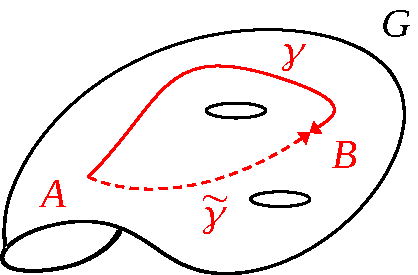
\includegraphics[width=1\linewidth]{images/arcwise_connected.pdf}
	\caption{Connected manifold.}
	\labfig{arcwise-connected}
\end{marginfigure}
\begin{definition}[Arcwise connected - \textit{Connesso per archi}]\index{Arcwise connected} A Lie group is \textbf{(arcwise) connected} if 
\[
\forall \ A,B\in G \ \ \exists \ \gamma:\comm{t_0}{t_1}\xrightarrow{C^0} G \ \ \text{ such that } 
\begin{cases}
    \gamma(t_0)=A\\
    \gamma(t_1)=B
\end{cases}
\]
\end{definition}\marginnote[-10mm]{Dal momento che ci è sembrata pià chiara, riportiamo anche la definizione di \textit{identity component} presente nel libro di Hall \cite{Hall2015}:
\begin{definition}[Identity component - Hall]For any matrix Lie group $G$, the \textbf{identity component} of $G$, denoted $G_0$, is the set of $A\in G$ for which there exists a continuos path $A(t)$, $a\leq t \leq b$, lying in $G$ with\footnote{$I$ is the neutral element} $A(a)=\textrm{I}$ and $A(b))A$.

\end{definition}}
\begin{definition}[Identity component]\index{Identity component} Given a Lie group\footnote{In general not connected} $G$, the \textbf{identity component} $G_0$ is the connected component containing the neutral element ($=\mathbb{1}$ for m.L.g.).
\end{definition}
\begin{marginfigure}[15mm]
	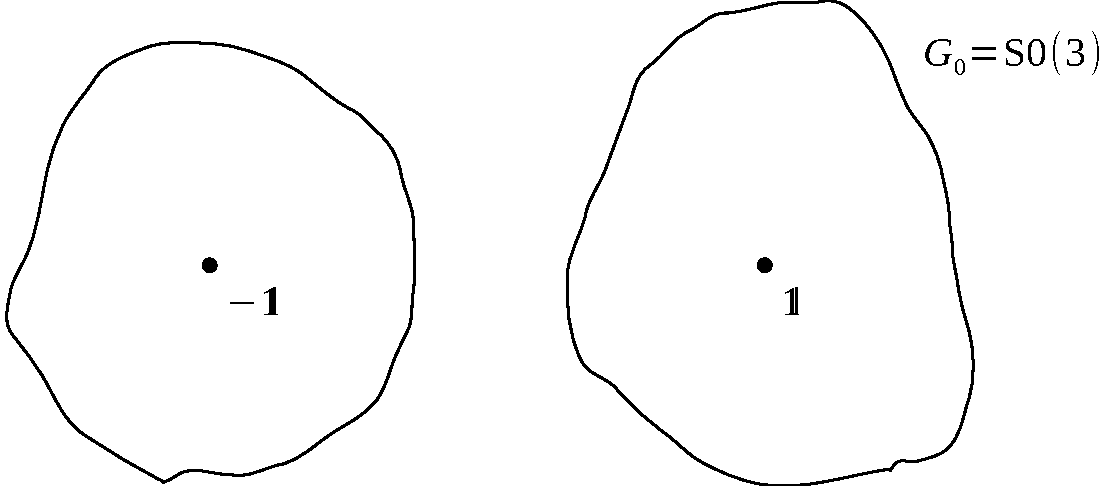
\includegraphics[width=1.2\linewidth]{images/Identity_component.pdf}
	\caption{}
	\labfig{Identity-component}
\end{marginfigure}
\begin{example}
\( \textrm{O}(3)=\Bqty{R\in\textrm{End}(\mathbb{R}^3): \ RR^T=\mathbb{1}=R^TR}\). Since
\[
R\in\textrm{O}(3) \quad \Rightarrow \quad \det(R)^2=\det(RR^T)=\det(\mathbb{1})=1
\]
And since we are using real numbers (there is no modulus) there are two connected components: on one hand there is the identity with determinant one, and the other hand there is minus the identity. And the connected component $G_0$ is what we call $\textrm{SO}(3)$. Notice that $\textrm{SO}(3)\trianglelefteq \textrm{O}(3)$ (\textbf{normal}). It can easily be checked by taking $R\in \textrm{SO}(3)$ and $S \in \textrm{O}(3)$ and taking
\[
\det\pqty{SRS^{-1}}=\det(S)\det(R)\det\pqty{S^{-1}}=\det(R)=1
\]
Then
\[
SRS^{-1}\in \textrm{SO}(3) \quad \forall \ R \in \textrm{SO}(3) \quad S \in \textrm{O}(3)
\]
Which means exactly that $\textrm{SO}(3)$ is not just a subgroup, but is a normal subgroup (it is left invariant by inner automorphism).\marginnote{Remember that normal subgroup are important because the quotient is still a group.}Then, the quotient is a group, indeed 
\[
{\color{red}\frac{\textrm{O}(3)}{\textrm{SO}(3)}=\Bqty{+\mathbb{1},-\mathbb{1}}\simeq\Bqty{+1,-1}}
\]
\end{example}
This fact that is very clear and explicitly in the case of rotations, it is actually a very general phenomenon.
\begin{theorem}[Identity component is a \textbf{normal subgroup}]\index{Identity component}Let $G$ be a Lie group, and $G_0$ its \textbf{identity component.} Then $G_0$ is a \textbf{normal Lie subgroup} of $G$, and hence $\nicefrac{G}{G_0}$ is a group.
\end{theorem}
\begin{proof}
\begin{marginfigure}
	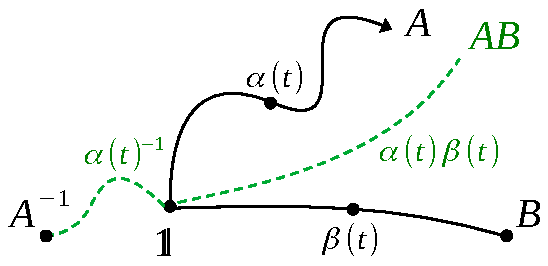
\includegraphics[width=1.1\linewidth]{images/id-is.norm-sub.pdf}
	\caption{Identity component of a normal subgroup}
	\labfig{id-is.norm-sub}
\end{marginfigure}
\begin{enumerate}
    \item $G_0\trianglelefteq G$. Take $A,B\in G_0$ and prove that $AB$ and $A^{-1}$ are still in $G_0$. This means (\reffig{id-is.norm-sub}) that there exists a continuous path $\alpha$ from the identity\sidenote{identity will be always used as synonymous of neutral element, because in the end we will apply everything to matrix Lie groups.} to $A$ and there is another continuous path $\beta$ from the identity to $B$ and we parameterize them as:
    \[
    \begin{split}
    \alpha:\comm{0}{1}\xrightarrow{{\color{red}C^0}} G \qquad &\alpha(0)=\mathbb{1}, \alpha(1) = A\\
    \beta:\comm{0}{1}\xrightarrow{{\color{red}C^0}} G \qquad &\beta(0)=\mathbb{1}, \beta(1) = B
    \end{split}
    \]
    What we can do is to multiply them, taking the path which at every time will be $\alpha(t)\beta(t)$ and it will be somewhere else. This path is still continuous because $\alpha$ and $\beta$ are continuous paths and the composition is smooth: at time zero it is still the identity (because identity times identity is the identity) and at time one it will be in $AB$. We can play the same game with the path $\alpha(t)^{-1}$, this is still a continuous path (because $\alpha$ is continuous and the inversion is smooth in a Lie group): at time $t=0$ it is in the identity and at time $t=1$ will be in $A^{-1}$. Hence
    \[
    \begin{split}
    \alpha\cdot\beta:\comm{0}{1}\xrightarrow{{\color{red}C^0}} G \quad &\textrm{connects} \ \mathbb{1} \textrm{ and } AB\\
    \alpha^{-1}:\comm{0}{1}\xrightarrow{{\color{red}C^0}} G \quad &\textrm{connects} \ \mathbb{1} \textrm{ and } A^{-1}
    \end{split}
    \]
    So there exists a continuous path from the identity to $AB$ and another from the identity to $A^{-1}$, so $AB\in G_0$ and $A^{-1}\in G_0$, which proves that $G_0$ is a subgroup.
    \begin{marginfigure}[-15mm]
	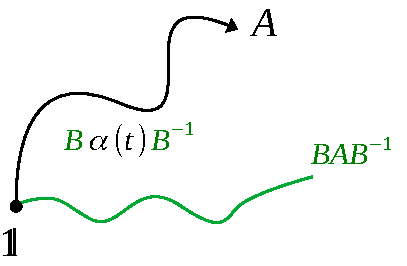
\includegraphics[width=1.1\linewidth]{images/id-is.norm-sub_proof.pdf}
	\caption[Sketch for the proof that identity component is a normal subgroup]{}
	\labfig{id-is-norm-sub-proof}
    \end{marginfigure}
    \item Now we want to prove that is a \textbf{normal} subgroup: $G_0\, {\color{red}\trianglelefteq}\, G$ ({\color{red}normal}). Take $A\in G_0$ and $B\in G$ and prove that $BAB^{-1}$ is in $G_0$. Since we know that $A\in G_0$ we know there is a continuous path from the identity to $A$, that we call $\alpha$, as in \reffig{id-is-norm-sub-proof}. Now we can take the sandwich (= conjugation) with $B$. At time $t=0$ it will be $BB^{-1}=\mathbb{1}$ and at time $t=1$ it will be $BAB^{-1}$:
    \[
    B\alpha(\cdot)B^{-1}: \comm{0}{1}\to G \quad
    \begin{cases}
    t=0 & \mathbb{1}\\
    t=1 & BAB^{-1}
    \end{cases}
    \]
    It is continuous because the operations are continuous and $\alpha$ was continuous.\marginnote[-21mm]{$B$ is fixed and multiplication times a fixed element is a continuous operation (in ???) a smooth Lie group.} Hence $BAB^{-1}$ is in $G_0$.
    \item $G_0$ is \textbf{closed} in $G$.\marginnote[-13mm]{To prove that is a Lie subgroup we use the Cartan's criterion  \ref{thm:CartanCriterion}, each connected component is both close and open. We should use something that we skipped: the fact that arcwise connected is equivalent to connected for a Lie group (in general for a manifold). If we go back to analysis I and II, we see that the definition of a connected set is a set which is both open and close in itself, this means that a connected component is both open and close in the ambient space, so it is closed. But a closed subgroup is a Lie subgroup} (because a connected component is both \textbf{open} and \textbf{closed}). Hence by Cartan's criterion [\vrefthm{CartanCriterion}] is a \textbf{Lie subgroup}.
\end{enumerate}
\end{proof}
As in the prototype example (the one of the rotation group) we have the same phenomenon in general: the identity component of a Lie group is a normal Lie subgroup and the quotient will be a group. Typically, in all the examples we are interested in, it will be a discrete group, as it happens for the rotations.

Which of the interesting groups are connected and which are not? A theory helps us.
%1:41:03
%INIZIO LEZIONE 22/04
\begin{theorem}
$\text{GL}(n,\mathbb{C})$ is \textbf{connected} for all $n\ge 1$.
\end{theorem}
\marginnote{From \textit{Capitolo 8 - Cambiamenti di base} of \cite{abate2006geometria}:

\textbf{Definizione.} Due matrici quadrate $A,A'\in M_{n,n}(\mathbb{K})$ dello stesso ordine si dicono \textit{simili}\index{Similar matrices} se esiste una matrice $B\in\textrm{GL}$ tale che $A'=B^{-1}AB$ (e quindi $A=BA'B^{-1}=\left(B^{-1}\right)^{-1}A'B^{-1}$).

\textbf{Proposizione.} Sia $T:V\to V$ un endomorfismo, $\pazocal{B}$ una bse di $V$ e $A$ la matrice associata a $T$ rispetto a $\pazocal{B}$. Allora se $\pazocal{B}'$ è un'altra base di $V$, la matrice $A'$ associata a $T$ rispetto a $\pazocal{B}'$ è simile ad $A$.}
\begin{example}Let us see why $\mathbb{C}$ is crucial with some examples:

\underline{$n=1$}: $\text{GL}(1,\mathbb{C})=\mathbb{C}^x$

But if we go to the real case: 

\underline{$n=1$}: $\text{GL}(1,\mathbb{R})=\mathbb{R}^x=(-\infty,0)\cup(0,+\infty)$, has 2 connected components!
\end{example}
%Fine LEZIONE  13 21/04/2022
\begin{proof}
We know from linear algebra that every matrix with complex entries $A\in\text{Mat}(n,\mathbb{C})$ is similar to an \textbf{upper diagonal matrix}, i.e. $\exists\,S\in \text{GL}(n,\mathbb{C})$ such that $A=SBS^{-1}$, with $B$ defined as:
\[
B=
\begin{pNiceArray}{ccc}[margin]
\lambda_1 & & *_B\\ 
 & \ddots & \\
 0 & & \lambda_n 
\end{pNiceArray}
\quad \text{where } \{\lambda_1,\dots,\lambda_n\} \text{ are eigenvalues of $A$ (and of $B$).}
\]
Consider now $A\in\text{GL}(n,\mathbb{C})$ and define a \textbf{deformation path in}\index{Deformation path} $\textrm{GL}(n,\mathbb{C})$ for $t\in[0,1]$:
\begin{marginfigure}
	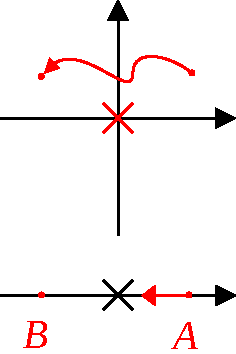
\includegraphics[width=1\linewidth]{images/ex-gl-conn.pdf}
	\caption[$\textrm{GL}(n,\mathbb{C)}$ is connected]{In simple words, if we are in $\mathbb{C}^\times$, we can go from one point to the other with a continuous path avoiding the origin; but if we are in $\mathbb{R}^\times$ we cannot.}
	\labfig{ex-gl-conn}
\end{marginfigure}
\[
\beta(t)=
\begin{pNiceArray}{ccc}[margin]
\lambda_1 & & (1-t)*_B\\ 
 & \ddots & \\
 0 & & \lambda_n 
\end{pNiceArray}
\quad
\begin{cases}
\beta(0)=B \\
\beta(1)=\text{diag}(\lambda_1,\dots,\lambda_n)\cong :D
\end{cases}
\]
where all the elements of the upper triangle corner of the matrix $\ast_B$ have been multiplied by $(1-t)$. At every $t$ we are in the general linear group, because
\[
\text{det}\beta(t)=\lambda_1\cdot\dots\cdot\lambda_n=\text{det}A\ne0\ \Rightarrow \ \beta:[0,1]\xrightarrow[]{{\color{red}C^0}}\text{GL}(n,\mathbb{C})
\]
\begin{figure*}[h!]
    \centering
    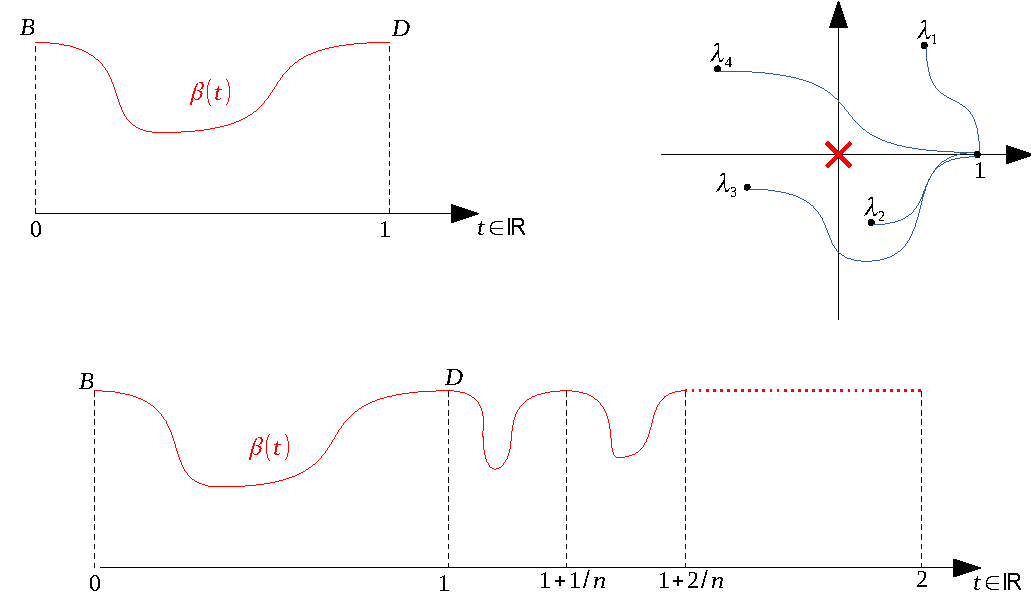
\includegraphics{images/deformation.pdf}
    \caption[Proof of a theorem for the connectness of GL]{$t$ is the pseudotime (not the physical one). On the upper right are represented the eigenvalues of the diagonal matrix on the complex plane.}
    \labfig{deformation}
\end{figure*}

\noindent Let us see the \reffig{deformation}.  On the upper right are represented the eigenvalues of the diagonal matrix on the complex plane, constrained by the fact that the determinant is different from zero (therefore each one of them should be different from zero). In each step, we deform an eigenvalue to 1 via a continuous path $\gamma_n(t)$, always avoiding the zero in some way. Then we divide the time to complete our process in $n$ steps as represented in the figure below:
\[
\textrm{First step:} \quad t\in[1,1+1/n]: 
\begin{pNiceArray}{ccc}[margin]
\gamma_1(t) & & 0\\ 
 & \ddots & \\
 0 & & \lambda_n 
\end{pNiceArray}
\]
Consider now the path $S\beta(t)S^{-1}$, for $t\in[0,2]$.
\begin{align*}
S\beta(t)S^{-1}:[0,2]&\xrightarrow[]{}\text{GL}(n,\mathbb{C})\\
A=SBS^{-1}&\mapsto S\mathbb{1}S^{-1}=\mathbb{1}
\end{align*}
It is continuous because it is the concatenation of finite number of continuous paths. This proves that \textbf{any} {\color{red}$A\in \text{GL}(n,\mathbb{C})$} is \textbf{arcwise connected to} $\mathbb{1}$. If now we consider $A,\Tilde{A}\in \text{GL}(n,\mathbb{C})$ we see that $A$ and $\Tilde{A}$ are arcwise connected in $\text{GL}(n,\mathbb{C})$.
\begin{marginfigure}[-50mm]
	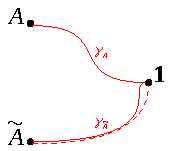
\includegraphics[width=1\linewidth]{images/connected.pdf}
	\caption{$A$ and $\Tilde{A}$ are both arcwise connected to $\mathbb{1}$, hence $A$ and $\Tilde{A}$ are arcwise connected.}
	\labfig{connected}
\end{marginfigure}
\end{proof}
With the same strategy (starting with the fact that $A$ is similar to upper triangular matrix, we deform the upper triangle to be zero and we get a diagonal), we can prove that also $\text{SL}(n, \mathbb{C})$ is connected, but this time we have the constraint that the product of all the eigenvalues must be equal to 1, therefore we have to move them either simultaneously or in pairs, because we have to find an arc inside the special linear group. This concept is emphasized in \reffig{constrain-sl-arc-conn}.
\begin{theorem}
$\text{SL}(n,{\color{red}\mathbb{C}})$ is \textbf{(arcwise) connected}.
\end{theorem}
\underline{\textbf{Visualization:}}
\begin{figure}[h!]
    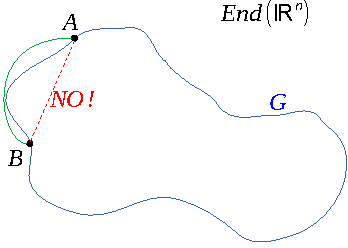
\includegraphics[width=0.5\textwidth]{images/NOSasso.pdf}
    \caption{Visualization of the constrain in $\textrm{SL}(n,\mathbb{C})$. The green line is supposed to be overlapped with the blue line.}
    \labfig{constrain-sl-arc-conn}
\end{figure}
$\gamma(t)_{\textrm{false}}=A(1-t)+Bt$ in End($\mathbb{R}^n$) it always exists.
\begin{theorem}
U(n) is \textbf{(arcwise) connected}
\end{theorem}
\begin{proof}
We know from linear algebra\marginnote[-1mm]{Cap. 11 (pag. 252 - esercizio per il lettore) of \cite{lang1985algebra}:

Un operatore $A: V\to V$ viene detto \textit{normale} quando $A^\ast A = AA^\ast$.

\textbf{Teorema (spettrale):}\index{Teorema spettrale} Sia $V$ uno spazio vettoriale di dimensione finita maggiore di zero sul corpo dei numeri complessi. Sia $\langle\;,\;\rangle$ una forma hermitiana definita positiva assegnata su $V$. Sia $A:V\to V$ un'applicazione lineare (detto anche operatore) normale. Esiste allora una base ortogonale di $V$ costituita da autovettori di $A$.

Il teorema si applica, dunque, anche al caso di applicazioni unitarie e viene enunciato dall'autore dello stesso libro a pagina 238 del capitolo 10. \textbf{Corollario}: Sia $A$ una matrice unitaria complessa. Esiste allora una matrice unitaria $U$ tale che $U^{-1}AU$ sia una matrice diagonale (pagina 239 Capitolo 10 di \cite{lang1985algebra})
 
Ogni autovalore di una matrice complessa unitaria $A$ si può scrivere come $e^{i\theta}$, per un opportuno numero reale $\theta$ (esercizio per il lettore da pagina 240 Capitolo 10 di \cite{lang1985algebra}).

From \href{https://en.wikipedia.org/wiki/Normal_operator}{Wikipedia}: examples of normal operators are
\begin{itemize}
    \item \textbf{unitary operators}: $N^\ast = N^{-1}$;
    \item \textbf{Hermitian operators} (i.e., self-adjoint operators): $N^* = N$
    \item \textbf{Skew-Hermitian} operators: $N^* = -N$
    \item \textbf{positive operators}: $N = MM^\ast$ for some $M$ (so $N$ is self-adjoint).
\end{itemize}}
that every $U$ unitary in End($\mathbb{C}^n)$ can be \textbf{ortho-diagonalized}, i.e. $\exists$ ortho-normal basis $\{e_1,\dots,e_n\}$ consisting of \textbf{eigenvectors of} $U$: 
\[
Ue_j=\underset{\mathclap{\tikz \node {$\uparrow$} node [below=1ex] {\footnotesize eigenvelue};}}{e^{i\theta_j}}\overset{\mathclap{\tikz \node {$\downarrow$} node [above=1.25ex] {\footnotesize eigenvector};}}{e_j} \qquad j\in\{1,\dots,n\}
\]
\noindent With the help of the ortho-normal basis, we can construct another unitary matrix $W\in\text{U}(n)$ which diagonalizes $U$, namely such that:
\[
WUW^{-1}=\begin{pNiceArray}{ccc}[margin]
e^{i\theta_1} & & 0\\ 
 & \ddots & \\
 0 & & e^{i\theta_n}
\end{pNiceArray}=D \quad \Rightarrow \quad U=W^{-1}DW
\]
Now we introduce a \textbf{deformation path} for $t\in[0,1]$ to make each eigenvalue one, while remaning unimodular:
\[
u(t)=W^{-1}\begin{pNiceArray}{ccc}[margin]
e^{{\color{red}i(1-t)}\theta_1} & & 0\\ 
 & \ddots & \\
 0 & & e^{{\color{red}i(1-t)}\theta_n}
\end{pNiceArray}W
\]
We have to check that:
\begin{enumerate}
    \item $u(0)=U$;
    \item $u(1)=\mathbb{1}$;
    \item $u(t)\in \textrm{U}(n)\  \forall t\in[0,1]$ because it is orthogonal and all the eigenvalues are uni-modular $\textrm{U}(1)$.
\end{enumerate}
\end{proof}
\begin{theorem}
SU$(n,\mathbb{C})$ is \textbf{arcwise connected.}
\end{theorem}
\begin{proof}
Similar ideas as before.
\end{proof}
\subsection{Simple connectedness}
\begin{definition}[Simply connected]{\index{Simply connected}}
A Lie group (in general, a manifold) is \textbf{simply connected} if it is \textbf{connected} and every \textbf{continuous loop} in G can be \textbf{"continuously deformed in G to a point".}
\end{definition}
\begin{figure}[h!]
    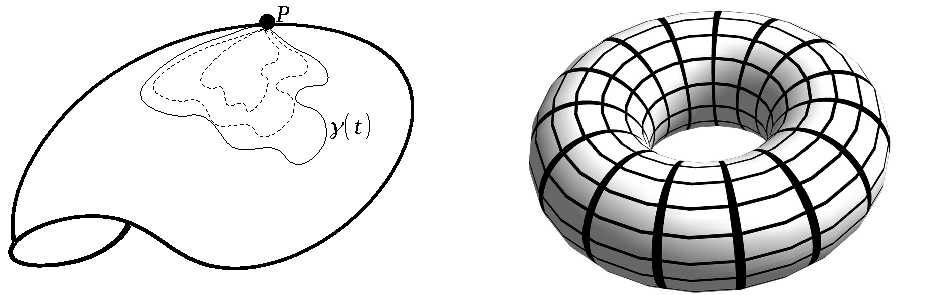
\includegraphics[width=\textwidth]{images/simplyconnected.pdf}
    \caption{The manifold on the left is simply connected, the torus on the right is not.}
    \labfig{man-simply-conn}
\end{figure}
The formal definitions is based on the fact that we have two pseudo-times: $t$ is the time of rotation and $s$ is the deformation of the loop. Formally, "can be continuously deformed in G to a point" means: 
\begin{align*}
\exists \ \sigma:[0,1]\times[0,1]&\xrightarrow[]{{\color{red}C^0}}\text{G}\\
(s,t)\quad &\mapsto\sigma(s,t)
\end{align*}
such that:
\begin{enumerate}
    \item $\sigma(0,t)=\gamma(t)\qquad \forall \ t\in[0,1]$
    \item $\sigma(s,0)=\sigma(s,1)\quad \forall \ s\in[0,1]$ \textbf{ "always loop"}
    \item $\sigma(1,t)=\sigma(1,0)\quad \forall \;\ t\in[0,1]$ \textbf{ "deformed to a point"}
\end{enumerate}
\end{document}